\chapter{Introdução}\label{Introducao}

A preservação e estudo do patrimônio arqueológico representam um campo de pesquisa crucial para a compreensão da história e cultura dos povos antigos. Entre esses vestígios históricos, as pinturas rupestres emergem como testemunhos tangíveis da arte e vida desses antigos grupos humanos (GUIMARÃES, 2013).

%Porque é crucial? porque é importante? Refita nessas questões.
%Sistemas de contagem, cultura de subsistência, compreender e adaptar as técnicas utilizadas para vida atual, Perspectiva social filosófica, estudar e entender o passado é uma maneira de entender quem nós somos. Cultura visual(não pensa o porque, mas o pra quê.)
%Essa ideia cultural cria uma alienação muito grande. Estamos nos aproprianado dos elementos da história da arte fora dos contextos de pensamento, de discussão. Não dá pra pensar as pinturas rupestres exclusivamente a partir delas. Quem atribui o nome arte pra aquilo somos nós. Não fazemos ideia se aqueles caras chamavam de arte ou pensavam nisso dessa forma. 

% Fazer um paralelo do novo com o antigo
% Começar contextualizando.
% O primeiro parágrafo é a contextualização do problema no mundo
% No século XXI, temos várias tecnologias obliquas e pervasivas presentes no mundo. Temos Inteligência Artifical, tecnologias novas surgindo o tempo todo. Mas e a nossa história? E as coisas antigas? Estamos esquecendo elas?
% O legal é que podemos juntar e usar a tecnologia a nosso favor para resgatar o passado e preservá-lo. 

Em Formosa-GO, o sítio arqueológico da Lapa da Pedra, popularmente conhecido como Toca da Onça, destaca-se pela presença de um conjunto significativo de pinturas rupestres, oferecendo \textit{insights} valiosos sobre a expressão artística e práticas culturais dos povos que habitaram essa área em tempos remotos.
    
Baseado nisso, este trabalho propõe uma abordagem inovadora para a preservação e divulgação das pinturas rupestres da Toca da Onça, integrando os avanços da arqueologia virtual e tecnologias de virtualização imersiva. O objetivo central é desenvolver uma plataforma de acesso público que não apenas documenta digitalmente as pinturas, mas também proporcione uma experiência interativa para os interessados em explorar esse patrimônio cultural de forma remota.

A criação de tal plataforma envolve desafios relacionados à criação de um \textit{website} para armazenar as informações sobre as pesquisas em arqueologia e sítios da cidade de Formosa, que permita aos usuários examinar as pinturas em detalhes, compreender seu contexto histórico e cultural, além de fornecer uma interface informativa. Paralelamente, busca-se desenvolver ambiente virtual imersivo para Windows, permitindo uma experiência de imersão mais profunda na análise das pinturas rupestres da Toca da Onça, que foi disponibilizado para \textit{download} no site desenvolvido. 

Para contextualizar, a preservação digital de sítios arqueológicos é uma prática essencial para garantir o acesso e a conservação de registros históricos e culturais de importância inestimável. No contexto da arte rupestre, métodos avançados, como a fotogrametria\footnote{A fotogrametria é uma técnica que utiliza fotografias para realizar medições precisas de objetos ou ambientes, permitindo a reconstrução tridimensional (3D). É explicada detalhadamente na Seção \ref{sec:fotogrametria e modelagem 3D} do Referencial Teórico.} e o uso de ambientes virtuais, têm sido empregados para criar representações digitais precisas de obras que, ao longo do tempo, se encontram ameaçadas pela degradação natural e pela ação humana.

O site original (Figura \ref{fig:Captura de tela da página inicial do blog}), desenvolvido no Blogger, desempenhou um papel fundamental na documentação e disseminação das pesquisas de Iniciação Científica realizadas pelo professor de Artes do Instituto Federal de Educação, Ciência e Tecnologia de Goiás (IFG) sobre o sítio arqueológico do Bisnau. O Blogger, uma plataforma criada em 1999, revolucionou a forma como as pessoas compartilhavam conteúdo online ao democratizar o acesso à publicação digital, permitindo que qualquer pessoa, independentemente de conhecimentos técnicos avançados, pudesse criar e manter um espaço virtual. Essa ferramenta foi essencial para dar visibilidade ao trabalho inicial do professor Edson, consolidando um importante repositório de informações sobre o patrimônio cultural da região.

Contudo, com o avanço das tecnologias digitais e as crescentes demandas por recursos mais robustos e personalizáveis, surgiu a necessidade de migrar para uma nova plataforma. O novo site não apenas preservará o legado do trabalho já realizado, como também ampliará seu alcance ao incluir novas pesquisas e registros sobre a Lapa da Pedra, além de incluir funcionalidades modernas. Essa transição permitirá uma melhor organização do conteúdo, maior interatividade e otimização para diferentes dispositivos, facilitando ainda mais o acesso e a disseminação desses estudos para a comunidade acadêmica e o público em geral.

\begin{figure}
    \centering
    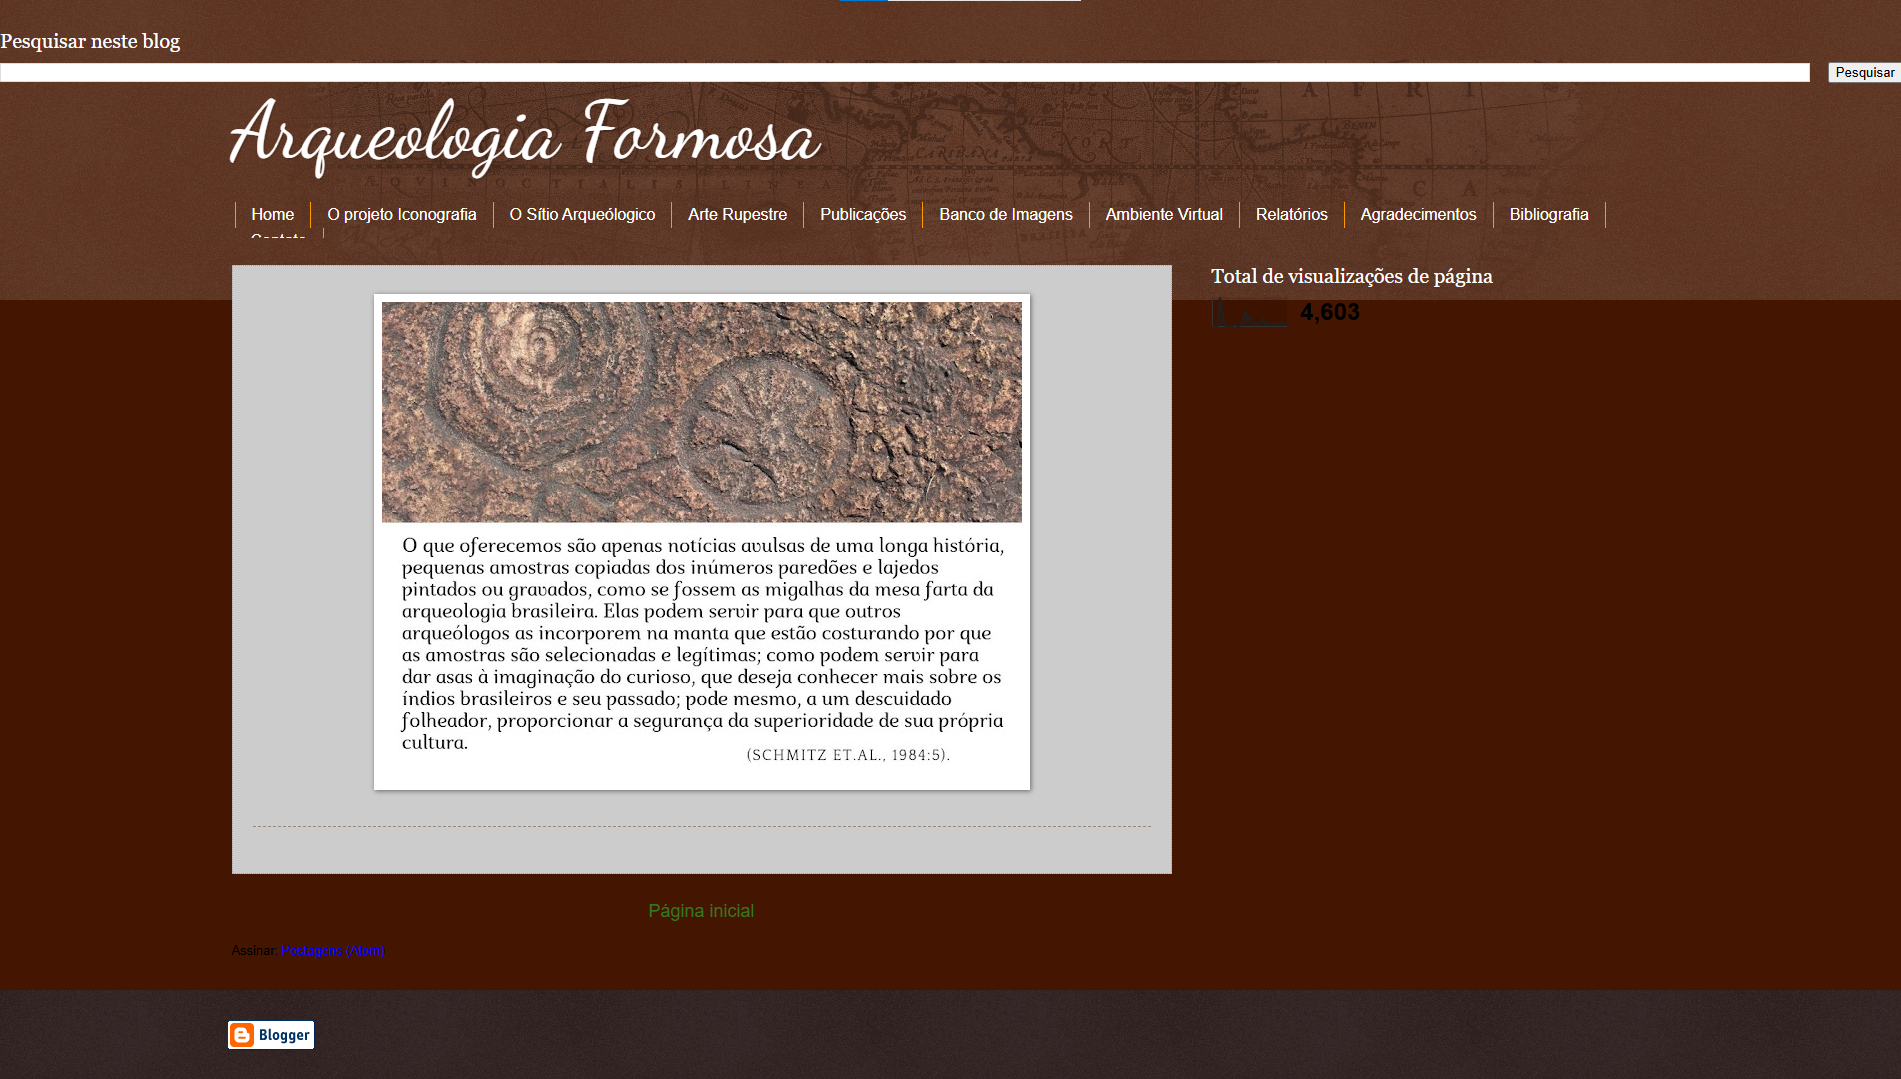
\includegraphics[width=1\linewidth]{images/home-blog-print.png}
    \caption{Captura de tela da página inicial do blog \href{https://arqueologiaformosa.blogspot.com/}{"Arqueologia Formosa"}}
    \label{fig:Captura de tela da página inicial do blog}
\end{figure}

\section{Objetivo Geral}
Desenvolver uma plataforma web e um ambiente virtual tridimensional (3D) interativo para preservar, divulgar e democratizar o acesso à arte rupestre da Lapa da Pedra, promovendo a conscientização sobre a importância desses registros culturais para educadores, pesquisadores e o público em geral.

\section{Objetivos Específicos}
Os objetivos específicos do projeto incluem:
\begin{itemize}
    \item Realizar uma análise heurística de usabilidade do antigo site "Arqueologia Formosa", a fim de identificar possíveis melhorias que otimizem a experiência do usuário e garantam uma navegação mais intuitiva e acessível.
    \item Desenvolver um novo site com um design centrado na experiência do usuário, do inglês, \gls{ux}, oferecendo navegação e acessibilidade aprimoradas.
    \item Implementar um ambiente virtual \gls{3d} que permita a visualização interativa da arte rupestre encontrada na Lapa da Pedra e disponibilizar para \textit{download} no site desenvolvido.
    \item Disponibilizar o ambiente virtual 3D para download no novo site, possibilitando que usuários explorem o conteúdo offline e em diferentes dispositivos.
    \item Contribuir para a educação patrimonial e a preservação digital do patrimônio cultural da região de Formosa, servindo como modelo replicável para outros sítios arqueológicos.
\end{itemize}


\section{Justificativa}
A relevância deste estudo está intrinsecamente relacionada à crescente importância da arqueologia virtual como uma ferramenta eficaz para a preservação e estudo do patrimônio arqueológico em um mundo que enfrenta desafios contínuos em relação à degradação dos sítios históricos. Neste contexto, tecnologias digitais não só oferecem uma nova forma de interagir com o passado, mas também permitem a democratização do acesso a elementos culturais. Por exemplo, projetos semelhantes têm demonstrado que a virtualização de artefatos históricos pode aumentar a conscientização e o respeito pelas culturas que moldaram nossa história.

Por outro lado, a criação de um ambiente digital para a preservação cultural traz inúmeras vantagens tanto para a educação quanto para a pesquisa, possibilitando o acesso a informações e experiências que, de outra forma, seriam limitadas. Além disso, a experiência prévia adquirida pelo autor no \gls{PIBIC} intitulado "Iconografia e Arte Rupestre Formosense: Criação de um Banco de Imagens e Modelos \gls{3D} da Lapa da Pedra" \footnote{Disponível para leitura em: 
\href{https://drive.google.com/file/d/1Id44ViPFScX0Z1TIxGngs4_7UXPabMDt/view?usp=sharing}{https://drive.google.com/file/d/1Id44ViPFScX0Z1TIxGngs4_7UXPabMDt/view?usp=sharing} *\textbf{ COLOCAR LINK DO SICT QUANDO FOR PUBLICADO}}, sob a orientação do professor de Artes do  Instituto Federal de Educação, Ciência e Tecnologia de Goiás (IFG), Edson Rodrigues Borges, enriqueceu significativamente a compreensão dos processos de fotogrametria e da criação de modelos 3D aplicados à arqueologia formosense. Com isso, esse conhecimento se torna fundamental para a implementação deste projeto, ao expandir e aprimorar o acesso a esses recursos digitais.

Dessa forma, esta pesquisa não apenas contribui para o avanço da arqueologia virtual, mas também possui implicações significativas na valorização e proteção do patrimônio cultural. Ao tornar acessíveis as pinturas rupestres da Toca da Onça a um público mais amplo, busca-se não só promover o conhecimento e a apreciação destes tesouros históricos, mas também engajar a sociedade na sua preservação, incentivando a reflexão sobre a identidade cultural e a herança coletiva que todos compartilhamos.

\section{Descrição dos Capítulos}
Os próximos capítulos deste trabalho são organizados da seguinte forma:
\begin{itemize}
    \item \textbf{Referencial Teórico}
    Dedica-se à fundamentação teórica do trabalho e aos principais conceitos e termos do trabalho, para que o leitor possa ter leitura fluida e compreensão integral do que está lendo. O capítulo aborda sobre a arqueologia e a arte rupestre, com foco no sítio Lapa da Pedra e nas ameaças à sua preservação. Discute o conceito de patrimônio virtual e suas aplicações, além dos métodos de fotogrametria, modelagem \gls{3d}, e práticas de engenharia de software e desenvolvimento web, com ênfase em Experiência do Usuário. Apresenta também as ferramentas utilizadas.
    
    \item \textbf{Método}: Explica o planejamento, a metodologia escolhida, a coleta de requisitos, o desenvolvimento do sistema, incluindo o uso de Kanban, a criação do ambiente virtual e o desenvolvimento do novo site.
    
    Descreve o processo de desenvolvimento adotado, incluindo a forma de organização das atividades (por exemplo, Kanban) e a coleta de requisitos. Expõe também a modelagem de dados e a arquitetura geral do sistema, explicando como cada componente foi planejado para atender aos objetivos.
    
    \item \textbf{Desenvolvimento}: Foca na implementação prática do projeto. Apresenta a construção do site com Next.js e Sanity, a integração com serviços externos (Flickr, Google Drive, Sketchfab) e, em seguida, o desenvolvimento do ambiente virtual na Unreal Engine, detalhando desde a 
    fotogrametria até a disponibilização do executável.
    
    \item \textbf{Resultados}: Descreve os produtos finais obtidos, comparando o novo site e o ambiente virtual com as versões anteriores.
    \item \textbf{Conclusão}: Resume os principais resultados alcançados, limitações encontradas e sugestões para trabalhos futuros.
    \item \textbf{Referências}: Lista as obras, artigos e demais fontes bibliográficas consultadas para embasar o trabalho.
    \item \textbf{Apêndice}: Reúnem materiais de apoio que não cabem no corpo principal, mas enriquecem o trabalho. Estão inclusos o questionário de requisitos, registros de reuniões, e demais documentos que auxiliam na compreensão detalhada do trabalho.


\end{itemize}

